\documentclass{beamer}
\mode<presentation> {
%\usetheme{Madrid}
%\usetheme{default}
\usepackage{color}
\definecolor{bottomcolour}{rgb}{0.21,0.11,0.21}
\definecolor{middlecolour}{rgb}{0.21,0.11,0.21}
\setbeamercolor{structure}{fg=white}
\setbeamertemplate{frametitle}[default]%[center]
\setbeamercolor{normal text}{bg=black, fg=white}
\setbeamertemplate{background canvas}[vertical shading]
[bottom=bottomcolour, middle=middlecolour, top=black]
\setbeamertemplate{items}[circle]

\setbeamertemplate{navigation symbols}{} %no nav symbols
\setbeamercolor{block title}{use=structure,fg=white,bg=structure.fg!50!red!50!blue!100!green}
\setbeamercolor{block body}{parent=normal text,use=block title,bg=block title.bg!5!white!10!bg,fg=white}
\setbeamertemplate{navigation symbols}{}
\newcounter{moncompteur}
}

\usepackage{graphicx} 
\usepackage{booktabs} 
\usepackage[utf8]{inputenc}  
\usepackage[T1]{fontenc}  
\usepackage{geometry}     
\usepackage[francais]{babel} 
\usepackage{eurosym}
\usepackage{verbatim}
\usepackage{ragged2e}
\justifying
%%%%%%%%%%%%%%%%%%%%%%%%%%%%%%%%%%%%%%%%%%%%%%%%%%%%%%%%%%%%%%%%
%% ccBeamer 0.1, 2007-07-02                                   %%
%% Written by Sebastian Pipping <webmaster@hartwork.org>      %%
%% ---------------------------------------------------------- %%
%% Licensed under Creative Commons Attribution-ShareAlike 3.0 %%
%% http://creativecommons.org/licenses/by-sa/3.0/             %%
%%%%%%%%%%%%%%%%%%%%%%%%%%%%%%%%%%%%%%%%%%%%%%%%%%%%%%%%%%%%%%%%


%% Images
\newcommand{\CcImageBy}[1]{%
	
\includegraphics[scale=#1]{creative_commons/cc_by_30.pdf}%
}
\newcommand{\CcImageCc}[1]{%
	
\includegraphics[scale=#1]{creative_commons/cc_cc_30.pdf}%
}
\newcommand{\CcImageDevNations}[1]{%
	
\includegraphics[scale=#1]{creative_commons/cc_dev_nations_30.pdf}%
}
\newcommand{\CcImageNc}[1]{%
	
\includegraphics[scale=#1]{creative_commons/cc_nc_30.pdf}%
}
\newcommand{\CcImageNd}[1]{%
	
\includegraphics[scale=#1]{creative_commons/cc_nd_30.pdf}%
}
\newcommand{\CcImagePd}[1]{%
	
\includegraphics[scale=#1]{creative_commons/cc_pd_30.pdf}%
}
\newcommand{\CcImageSa}[1]{%
	
\includegraphics[scale=#1]{creative_commons/cc_sa_30.pdf}%
}
\newcommand{\CcImageSampling}[1]{%
	
\includegraphics[scale=#1]{creative_commons/cc_sampling_30.pdf}%
}
\newcommand{\CcImageSamplingPlus}[1]{%
	
\includegraphics[scale=#1]{creative_commons/cc_sampling_plus_30.pdf}%
}


%% Groups
\newcommand{\CcGroupBy}[1]{% zoom
	\CcImageBy{#1}%
}
\newcommand{\CcGroupByNc}[2]{% zoom, gap
	\CcImageBy{#1}\hspace*{#2}\CcImageNc{#1}%
}
\newcommand{\CcGroupByNcNd}[2]{% zoom, gap
	\CcImageBy{#1}\hspace*{#2}\CcImageNc{#1}\hspace*{#2}\CcImageNd{#1}%
}
\newcommand{\CcGroupByNcSa}[2]{% zoom, gap
	\CcImageBy{#1}\hspace*{#2}\CcImageNc{#1}\hspace*{#2}\CcImageSa{#1}%
}
\newcommand{\CcGroupByNd}[2]{% zoom, gap
	\CcImageBy{#1}\hspace*{#2}\CcImageNd{#1}%
}
\newcommand{\CcGroupBySa}[2]{% zoom, gap
	\CcImageBy{#1}\hspace*{#2}\CcImageSa{#1}%
}
\newcommand{\CcGroupDevNations}[1]{% zoom
	\CcImageDevNations{#1}%
}
\newcommand{\CcGroupNcSampling}[2]{% zoom, gap
	\CcImageNc{#1}\hspace*{#2}\CcImageSampling{#1}%
}
\newcommand{\CcGroupPd}[1]{% zoom
	\CcImagePd{#1}%
}
\newcommand{\CcGroupSampling}[1]{% zoom
	\CcImageSampling{#1}%
}
\newcommand{\CcGroupSamplingPlus}[1]{% zoom
	\CcImageSamplingPlus{#1}%
}


%% Text
\newcommand{\CcLongnameBy}{Attribution}
\newcommand{\CcLongnameByNc}{Attribution-NonCommercial}
\newcommand{\CcLongnameByNcNd}{Attribution-NoDerivs}
\newcommand{\CcLongnameByNcSa}{Attribution-NonCommercial-ShareAlike}
\newcommand{\CcLongnameByNd}{Attribution-NoDerivs}
\newcommand{\CcLongnameBySa}{Attribution-ShareAlike}

\newcommand{\CcNote}[1]{% longname
	This work is licensed under the \textit{Creative Commons #1 3.0 License}.%
}

\title[Comment sécuriser sa messagerie mail?]{Comment sécuriser sa messagerie mail?} 
\author{Genma}
\begin{document}
%% Titlepage
\begin{frame}
	\titlepage
	\vfill
	\begin{center}
		\CcGroupByNcSa{0.83}{0.95ex}\\[2.5ex]
		{\tiny\CcNote{\CcLongnameByNcSa}}
		\vspace*{-2.5ex}
	\end{center}
\end{frame}

\begin{frame}
\frametitle{
\includegraphics[scale=0.4]{./Genma.jpg} \ \ \  A propos de moi  }
\begin{columns}[c] 

\column{.55\textwidth} 
\textbf{Où me trouver sur Internet?}
\begin{itemize}
\item Le Blog de Genma : http://genma.free.fr
\item Twitter : http://twitter.com/genma
\end{itemize}

\textbf{Mes centres d'intérêts?}
\\ Plein de choses dont:
\begin{itemize}
\item La veille technologique
\item Le chiffrement
\end{itemize}

\column{.5\textwidth} 
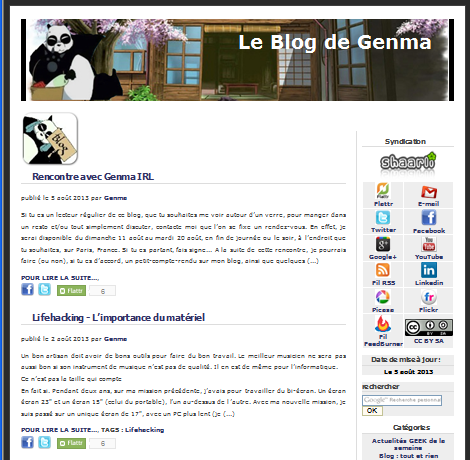
\includegraphics[width=5cm,height=5cm]{blog.png} 

\end{columns}
\end{frame}

%------------------------------------------------

\begin{frame}
\frametitle{But de cette présentation}

Cette présentation explique comment sécuriser sa messagerie mail.

\begin{block}{PLAN}
\begin{itemize}
\justifying{
\item Par défaut les mots de passe sont visibles.
\item Serveur de réception d'eMail IMAP.
\item Serveur d'envoi eMail (SMTP) authentifié.
\item Et pour le webmail? Connexion en https.
\item Et pour le contenu des mails? Chiffrement des mails avec PGP.
\item Et pour aller BEAUCOUP plus loin? SSL de bout en bout.
}
\end{itemize}
\end{block}
\end{frame}


%----------------------------------------------------------------------------------------
\begin{frame}
\frametitle{Par défaut les mots de passe sont visibles}

\begin{block}{\justifying{Comment éviter la transmission en clair des mots de passe avec les logiciels de messagerie?}}
\justifying{
Il est important de configurer son logiciel de messagerie de manière à éviter la transmission du mot de passe en utilisant des communications protégées par un protocole de chiffrement (TLS - Transport Layer Security, SSL - Secure Socket Laye).
}
\end{block}
\end{frame}


%----------------------------------------------------------------------------------------
\begin{frame}
\begin{center}
\Huge{Thunderbird et le paramétrage}
\end{center}
\end{frame}

%----------------------------------------------------------------------------------------
\begin{frame}
\frametitle{Serveur de réception d'eMail IMAP}

\begin{block}{Sécuriser l'accès à votre boite eMail IMAP grâce au protocole IMAP SSL}
\justifying{
Pour ce faire, depuis votre client de messagerie (Thunderbird), il suffit d'activer l'option de sécurité de votre connexion IMAP, dans les paramètres de compte. Le port utilisé est le 993.
}
\end{block}
\begin{center}
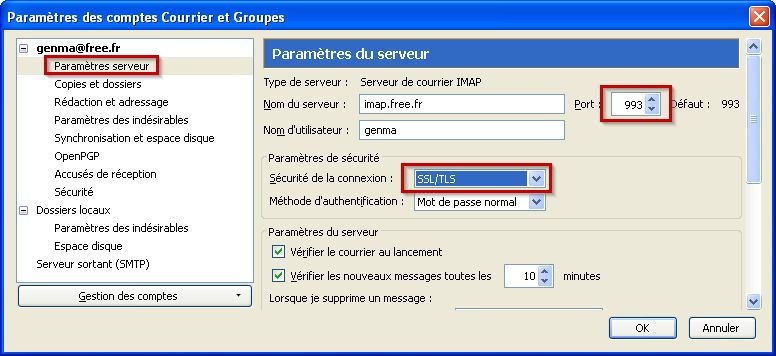
\includegraphics[scale=0.5] {./images/Thunderbird01.jpg}
\end{center}
\end{frame}

%----------------------------------------------------------------------------------------
\begin{frame}
\frametitle{Serveur d'envoi eMail (SMTP) authentifié}

\begin{block}{Sécuriser l'envoi de mail SMTP via SSL}
\justifying{
L'authentification SMTP avec sécurité de connexion en SSL (port 465) vous permet d'envoyer vos eMails (hors Webmail) depuis n'importe quelle connexion (par exemple lors de déplacements).\\ 
Avantage : il ne sera pas nécessaire d'adapter et d'utiliser le serveur de courrier sortant qui dépend du fournisseur Internet d'où vous vous trouvez.
\\ 
Cas de Free : nécessite d'activer l'authentification SMTP dans les paramètres de son compte.}
\end{block}
\end{frame}

%----------------------------------------------------------------------------------------
\begin{frame}
\frametitle{Serveur d'envoi eMail (SMTP) authentifié}

\begin{block}{Configuration de Thunderbird}
\justifying{
Pour ce faire, depuis votre client de messagerie (Thunderbird), il suffit de renseigner le champs Nom d'utilisateur par votre identifiant (login)  et de choisir SSL/TLS, port 465 pour la méthode de sécurité.
}
\end{block}
\begin{center}
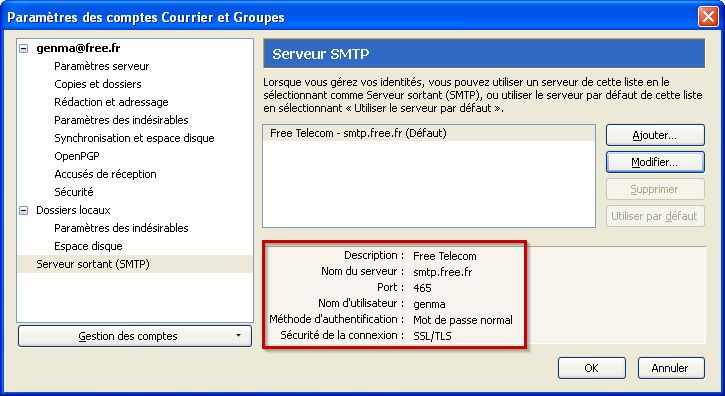
\includegraphics[scale=0.5] {./images/Thunderbird02.jpg} 
\end{center}

\end{frame}


%----------------------------------------------------------------------------------------
\begin{frame}
\begin{center}
\Huge{Et pour le webmail?}
\end{center}
\end{frame}


%----------------------------------------------------------------------------------------
\begin{frame}
\frametitle{Cas du webmail}

\justifying{
Utiliser la connexion en https.
}
\begin{center}
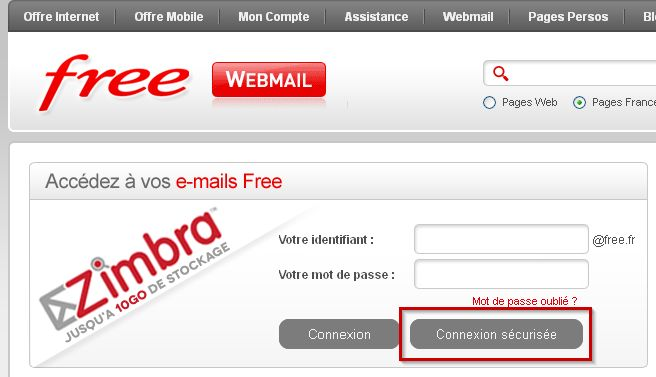
\includegraphics[scale=0.5] {./images/Webmail01.jpg}
\end{center}
\end{frame}

%----------------------------------------------------------------------------------------
\begin{frame}
\begin{center}
\Huge{Et pour le contenu des mails?}
\end{center}
\end{frame}

%----------------------------------------------------------------------------------------
\begin{frame}
\frametitle{Chiffrement des mails}

\begin{block}{Chiffrement des mails avec PGP}
\justifying{
Installer l'extension Enigmail et utiliser le chiffrement avec PGP.
\\
Voir les tutoriaux/conférences dédiés.
}
\end{block}
\begin{center}
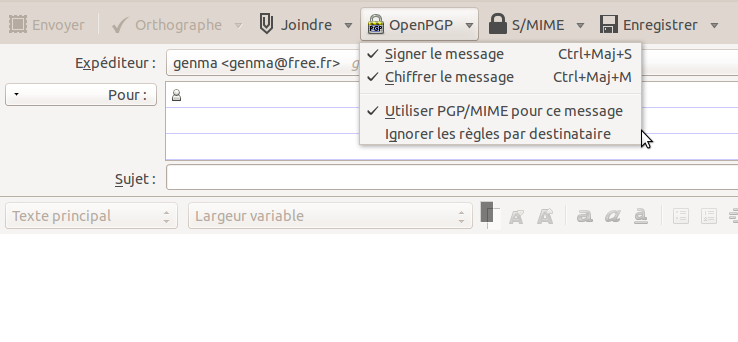
\includegraphics[scale=0.4] {./images/Thunderbird03.png}
\end{center}
\end{frame}

%----------------------------------------------------------------------------------------
\begin{frame}
\begin{center}
\Huge{Et pour aller BEAUCOUP \\plus loin?}
\end{center}
\end{frame}

%----------------------------------------------------------------------------------------
\begin{frame}
\frametitle{SSL de bout en bout}
\begin{block}{Un peu de théorie}
\justifying{Par défaut, en sortant du serveur de mail, le mail circule en clair jusqu'au serveur de mail destinataire.
Si le serveur d'envoi du mail se connecte en SSL au serveur destinataire, il y a établissement d'une connexion chiffrée.
On a donc :
}
\begin{itemize}
\justifying{
\item Client vers Serveur SMTP : connexion SSL
\item Serveur SMTP vers Serveur Mail destinataire : connexion SSL
\item Serveur IMAP vers client : connexion SSL
}
\end{itemize}
\end{block}
\justifying{
Conséquence : la connexion est chiffrée de bout en bout.
\\
Mais cela nécessite d'avoir son propre serveur, pour l'envoyeur et le destinataire du mail. 
}
\end{frame}

%----------------------------------------------------------------------------------------
\end{document}
